\chapter{Mathematical Formulation}
\label{chap:mipformulation}


%%%%%%%%%%%%%%%%%%%%%%%%%%%%%%%%%%%%%%%%%%%%%%%%%%%%%%%%%%%%%%%%%%%%%%%%%%%%%%%%%%

This chapter describes a method for solving the problem which is purely based on integer linear programming (ILP).

As mentioned by \cite{Haroldo2012}, since exact methods, which try to find proven optimal solutions, can demand unrealistic amounts of processing time on most timetabling variants, the development of heuristics which are effective in practice received much attention from researches.

At \cite{Birbas2009}: The lack of efficient software tools for the solution of IP models some years back has forced researchers away from suggesting standard IP solution techniques. Since the early 90's though, this obstacle has been removed and mathematical programming tools are contributing towards the effort of automating the timetabling process for high schools and for universities.

Section ~\ref{IP} introduces the main concepts of integer linear programming, which are fundamental in understanding the developed solving method. Further and more complete explanations about integer programming can be found at \cite{Wolsey98}.


%%%%%%%%%%%%%%%%%%%%%%%%%%%%%%%%%%%%%%%%%%%%%%%%%%%%%%%%%%%%%%%%%%%%%%%%%%%%%%%%%%
\section{Integer programming}
\label{IP}

A mathematical optimization problem consists of a set of equations which together define feasible solutions for a problem and an objective function that eliminates symmetries between these solutions and guides the search for the best solution.

When both objective function and constraints are linear, then it is called \textit{Linear Programming (LP)}.

$$
\begin{array}{rl}
   \mbox{Maximize} & c \cdot x
								\\ & A \cdot x \le b
								\\ & x \in \mathbb{R}^{n}_{+}
\end{array}
$$

where $A$ is a matrix such that $A \in \mathbb{R}^{m \times n}$, $c$ is a row vector such that $c \in \mathbb{R}^n$, $b$ is a column vector such that $b \in \mathbb{R}^m$, and $x$ is a column vector of decision variables.

Variations of a linear program are obtained when one constraints variables' domain. A \textit{Mixed Integer Program (MIP)} is a mathematical optimization in which some but not all variables are restricted to be integers. 

$$
\begin{array}{rlll}
   \mbox{Maximize} & c \cdot x & +  & h \cdot y
								\\ & A \cdot x & +  & G \cdot y \le b
								\\ & x \in \mathbb{R}^{n}_{+} &, & y \in \mathbb{Z}^{p}_{+}
\end{array}
$$

where $G$ is a matrix such that $G \in \mathbb{R}^{m \times p}$, $h$ is a row vector such that $h \in \mathbb{R}^p$, and $y$ is a column vector of integer decision variables.

When all decision variables must be integers, the program is called a \textit{Pure Integer Linear Program (IP)}; and when all decision variables are restricted to ${0,1}$ values, then we have a \textit{Binary Integer Program (BIP)}.

Very efficient methods for solving linear programs are known, with the Simplex Method being the most famous one. Because integer programs look pretty much like linear programs, it is not a surprise that linear programming theory and practice is essential in understanding and solving integer programs. Solving an integer program is far more challenging than solving its linear version though.

Since the integer set $\mathbb{Z}$ is a countable set, it is clear that every integer program has a countable number of solutions and that every bounded integer program has a countable and finite set of solutions. Thus, theoretically, these problems can be solved by enumeration. In practice, to be feasible, such approach depends on the size of the possible solutions set, and that is where difficulty stems from.

To illustrate the situation, consider a general assignment problem, where $n$ people are available to carry out $n$ jobs and each person must be assigned to carry out exactly one job. There is an one-to-one correspondence between assignments and permutations of ${1, \ldots ,n}$. Thus there are $n!$ solutions to compare. At table ~\ref{table:factorial} one can have a glimpse of what happens in this case when n grows.

\begin{table}[ht]
\caption{Combinatorial explosion of possible solutions for factorial function problems} % title of Table
\centering
\begin{tabular}{c c} 							% centered columns
\hline\hline 											% inserts double horizontal lines
$n$ & $n!$ \\ [0.5ex] 						% heading													
\hline 														% inserts single horizontal line
10 & $3.6 \cdot 10^6$ \\
100 & $9.33 \cdot 10^{157}$ \\
1000 & $4.02 \cdot 10^{2567}$ \\ [1ex] 	% [1ex] adds vertical space
\hline
\end{tabular}
\label{table:factorial} 					% is used to refer this table in the text
\end{table}


The obvious conclusion is that using complete enumeration for solving combinatorial problems, also known as \q{brute-force search} or \q{exhaustive search}, is feasible only for small values of $n$.



%%%%%%%%%%%%%%%%%%%%%%%%%%%%%%%
\subsection{Alternative formulations}

For every integer subset $X \subset \mathbb{Z}^n$ there is an infinite number of linear programs such that their feasible integer solution space is equal to $X$. Figure ~\ref{fig:linearForm} illustrates a subset $X \subset \mathbb{Z}^2$ of integer points and 3 different possible ways ($P_{1}$, $P_{2}$ and $P_{3}$) to linearly constrain the subset so that no integer point of $X$ is out of the bounded area and no integer point out of $X$ is inside the bounded area.

\begin{figure}[h]
\centering
\hfill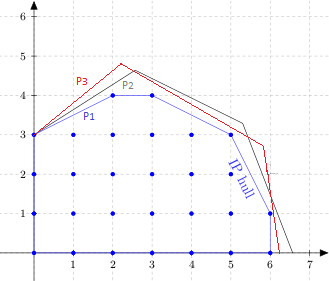
\includegraphics[scale=1.0]{figures/linearForm3.png}
\caption{Different linear formulations}
\label{fig:linearForm}
\end{figure}

Following are some useful definitions for the subject.

\paragraph{Definition}
A subset of $\mathbb{R}^{n}$ described by a finite set of linear constraints $P=\{x \in \mathbb{R}^{n}: Ax \le b\}$ is a \textit{polyhedron}.

\paragraph{Definition}
A polyhedron $P \subseteq \mathbb{R}^{n+p}$ is a \textit{formulation} for a set $X \subseteq \mathbb{Z}^{n} \times \mathbb{R}^{p}$ if and only if $X = P \cup (\mathbb{Z}^{n} \times \mathbb{R}^{p})$.

\vspace{7 mm}

Although all three formulations in figure ~\ref{fig:linearForm} are valid for definition of subset $X$, the formulation $P_{1}$ is ideal, because solving a linear program over $P_{1}$ leads to an optimal solution lying at an extreme point. Since each extreme point of $P_{1}$ is integer, it follows that the integer program is solved.

Generally speaking, given a set $X \subseteq \mathbb{R}^n$ and two formulations $P_{1}$ and $P_{2}$ for $X$, $P_{1}$ is a better formulation than $P_{2}$ if $P_{1} \subset P_{2}$. Formulation $P_{1}$ is said to be \textit{tighter} than $P_{2}$.



%%%%%%%%%%%%%%%%%%%%%%%%%%%%%%%
\subsection{Linear relaxation}




%%%%%%%%%%%%%%%%%%%%%%%%%%%%%%%
\subsection{Integrality gap}

Introduces integrality gap concept.

As in all combinatorial scheduling models, the problem grows more complex as the number of side constraints increases.\fixme{Colocar essa frase no lugar adequado!}


%%%%%%%%%%%%%%%%%%%%%%%%%%%%%%%
\subsection{Branch and Bound}

Introduces branch and bound concept.


%%%%%%%%%%%%%%%%%%%%%%%%%%%%%%%
\subsection{MIP Solver}

Introduces CPLEX and Gurobi.



%%%%%%%%%%%%%%%%%%%%%%%%%%%%%%%%%%%%%%%%%%%%%%%%%%%%%%%%%%%%%%%%%%%%%%%%%%%%%%%%%%
%%%%%%%%%%%%%%%%%%%%%%%%%%%%%%    TATIC MODULE     %%%%%%%%%%%%%%%%%%%%%%%%%%%%%%%
%%%%%%%%%%%%%%%%%%%%%%%%%%%%%%%%%%%%%%%%%%%%%%%%%%%%%%%%%%%%%%%%%%%%%%%%%%%%%%%%%%

\section{IP - Assignment Formulation}

The process of formulating an integer program can be organized in three steps:

\begin{enumerate}
\item Define what appear to be the necessary variables.
\item Use these variables to define a set of constraints so that the feasible points correspond to feasible solutions to the problem.
\item Use these variables to define the objective function.
\end{enumerate}

Usually the need of auxiliary variables arises while formulating constraints, which gives an iterative feature to the process until a consistent model is reached.


%%%%%%%%%%%%%%%%%%%%%%%%%%%%%%%%%%%%%%%%%%%%%%%%%%%%%%%%%%%%%%%%%%%%%%%%%%%%%%%%%%

\subsection{Notation}

%%%%%%%%%%%%%%%%%%%%%%%%%%%%%%%%%%%%%%%%%%
\subsubsection{Sets}

\begin{itemize}
\item $Al$ - Set of students. Elements of $Al$ are called $a$.
\item $C$ - Set of majors. Elements of $C$ are called $c$.
\item $CP$ - Set of campi. Elements of $CP$ are called $cp$.
\item $D$ - Set of courses. Elements of $D$ are called $d$.
\item $D_{a}$ - Set of courses required by student $a$.
\item $H_{t}$ - Set of time slots of day $t$. Elements of $H_{t}$ are called $h$.
\item $I_{d}$ - Set of sections of a course $d$. Elements of $I_{d}$ are called $i$.
\item $O$ - Set of majors offers. Elements of $O$ are called $oft$.
\item $S_{u}$ - Set of classrooms of block $u$. Elements of $S_{u}$ are called $s$.
\item $T$ - Set of weekdays. Elements of $T$ are called $t$.
\item $U$ - Set of blocks. Elements of $U$ are called $u$.
\item $SL$ - Set of calenders. Elements of $SL$ are called $sl$.
\item $P$ - Set of all professors. Elements of $P$ are called $p$.
\end{itemize}

%%%%%%%%%%%%%%%%%%%%%%%%%%%%%%%%%%%%%%%%%%
\subsubsection{Model Data}

\begin{itemize}
\item $Cap_{s}$ - Capacity of classroom $s$.
\item $nCreds_{d}$ - Total of credits of course $d$.
\item $duration_{h}$ - Total of minutes of time slot $h$.
\item $duration_{hi,hf}$ - Total of minutes from the beginning of time slot $hi$ to the end of time slot $hf$.
\item $M$ - big $M$.
\item $N_{d,k,t}$ - number of credits for course $d$ at day $t$ of credits split rule $k$.
\item $NCH_{d,hi,hf}$ - number of credits for course $d$ from time slot $hi$ to time slot $hf$.
\item $MinSize$ - minimum number of students required for offering a class.
\item $delta_{t,f}$ - maximum of idle time allowed at phase $f$ of day $t$ for a professor. Used only for gap-constraints, usually is the average sum of intervals at phase $f$ of day $t$ of calenders.
\item $pv$ - Unique virtual professor, to be used whenever the set of real professors is not enough for demand satisfaction.
\item $MinCredsDia_{a,t}$ - minimum number of credits expected for student $a$ at day $t$.
\end{itemize}

%%%%%%%%%%%%%%%%%%%%%%%%%%%%%%%%%%%%%%%%%%
\subsubsection{Variables}

\begin{itemize}
\item $v_{a,i,d,s,t,hi,hf}$ - binary variable, indicates if student $a$ is assigned to a class of section $i$ of course $d$, at classroom $s$, from time slot $hi$ to time slot $hf$ of day $t$. 
\item $x_{i,d,u,s,hi,hf,t}$ - binary variable, indicates if section $i$ of course $d$ is assigned to classroom $s$ from time slot $hi$ to time slot $hf$ of day $t$. 
\item $z_{i,d}$ - binary variable, indicates if section $i$ of course $d$ is offered. 
\item $o_{i,d,s}$ - binary variable, indicates if section $i$ of course $d$ is offered at classroom $s$. 
\item $fd_{d,a}$ - binary slack variable, indicates if student $a$ has his request for course $d$ not satisfied.
\item $fkm_{d,i,t}$ - slack variable for inferior limit for credits split rule constraint. 
\item $fkp_{d,i,t}$ - slack variable for superior limit for credits split rule constraint.
\item $m_{d,i,k}$ - binary variable, indicates if a credits split rule $k$ was chosen for section $i$ of course $d$.
\item $s_{i,d,a}$ - binary variable, indicates if student $a$ is assigned to section $i$ of course $d$.
\item $k_{p,i,d,u,h,t}$ - binary variable, indicates if professor $p$ teaches to section $i$ of course $d$ at block $u$ at time slot $h$ and day $t$.
\item $y_{p,i,d,cp}$ - binary variable, indicates if professor $p$ is assigned to section $i$ of course $d$ of campus $cp$.
\item $hip_{p,t,f}$ - integer variable, indicates the time in minutes of the first time slot assigned to professor $p$ at session $f$ of day $t$. For example, if the first class assigned to $p$ on $t=Monday$ and $f=morning$ starts at 9:30 am, then $hip_{p,t,f}=9\cdot 60 + 30 = 570$.
\item $hfp_{p,t,f}$ - integer variable, indicates the time in minutes of the end of the last time slot assigned to professor $p$ at session $f$ of day $t$.
\item $fpgap_{p,t,f}$ - integer slack variable, indicates the gap in session $f$ of day $t$ of professor $p$'s schedule.
\item $fcad_{a,t}$ - integer slack variable, indicates the number of credits bellow the expected assigned to student $a$ at day $t$.
\item $begin_{a,t,h}$ - binary variable, indicates if first class of student $a$ at day $t$ begin at time $h$.
\item $end_{a,t,h}$ - binary variable, indicates if last class of student $a$ at day $t$ begin at time $h$.
\item $at_{a,t}$ - binary variable, indicates if student $a$ has classes at day $t$.

\end{itemize}


%%%%%%%%%%%%%%%%%%%%%%%%%%%%%%%%%%%%%%%%%%%%%%%%%%%%%%%%%%%%%%%%%%%%%%%%%%%%%%%%%%
%%%%%%%%%%%%%%%%%%%%%%%%%%%%%%%%%%%%%%%%%%%%%%%%%%%%%%%%%%%%%%%%%%%%%%%%%%%%%%%%%%

\subsection{Formulation}


\subsubsection{Objective function}
$$
\begin{array}{rl}
   \mbox{MIN} &
			\sum\limits_{a \in A}\sum\limits_{d \in D} \cdot fd_{d,a}
      \\
      &
       + \sum\limits_{d \in D} 
\sum\limits_{t \in T} \sum\limits_{i \in I_{d}} (fkp_{d,i,k} + fkm_{d,i,k})
      \\
      &
       + \sum\limits_{a \in A} \sum\limits_{t \in T} fcad_{a,t}
      \\
      &      
      + \sum\limits_{p \in P} \sum\limits_{t \in T} \sum\limits_{f \in F} fpgap_{p,t,f}
      \\
      &
      + \sum\limits_{i \in I_{d}} \sum\limits_{d \in D} y_{pv,i,d,cp}
\end{array}
$$


%%%%%%%%%%%%%%%%%%%%%%%%%%%%%%%%%%%%%%%%%%%%%%%%%%%%%%%%%%%%%%%%%%%%%%%%%%%%%%%%%%
%%%%%%%%%%%%%%%%%%%%%%%%%%%%%%%%%%%%%%%%%%%%%%%%%%%%%%%%%%%%%%%%%%%%%%%%%%%%%%%%%%


\subsubsection{Assigns 'v' to 'x' and ensures classroom capacity}
\begin{eqnarray}
\sum\limits_{a \in A} v_{a,i,d,s,t,hi,hf}  \le Cap_{s} \cdot x_{i,d,s,t,hi,hf} \nonumber \qquad 
\\
\forall d \in D \quad
\forall i \in I_{d} \quad 
\forall s \in S \quad
\forall t \in T \quad 
\forall hi \in H \quad 
\forall hf \in H
\end{eqnarray}

\subsubsection{Assigns the classroom of a section to variable 'o'}
\begin{eqnarray}
M \cdot o_{i,d,s}  \geq \sum\limits_{t \in T}\sum\limits_{hi \in H}\sum\limits_{hf \in H} x_{i,d,s,t,hi,hf}  \nonumber \qquad 
\\
\forall d \in D \quad
\forall i \in I_{d} \quad
\forall u \in U \quad
\forall s \in S_{u} \quad
\end{eqnarray}

\subsubsection{Ensures single classroom per course section}
\begin{eqnarray}
\sum\limits_{u \in U} \sum\limits_{s \in S_{u}} o_{i,d,s}  \leq  z_{i,d,cp}  \nonumber \qquad 
\forall d \in D \quad
\forall i \in I_{d} \quad
\end{eqnarray}

\subsubsection{No overlapping in classroom's timetable}
\begin{eqnarray}
\sum\limits_{i \in I_{d}} \sum\limits_{d \in D} \sum\limits_{hi \in H_{d}} \sum_{\substack {hf \in H_{d} \\ hi\le hf}} x_{i,d,s,t,hi,hf}  \leq  1  \nonumber \qquad 
\\
\forall cp \in CP \quad
\forall u \in U_{cp} \quad
\forall s \in S_{u} \quad
\forall t \in T \quad
\forall h \in H \quad (hi,hf)\text{ overlaps }h
\end{eqnarray}

\subsubsection{Tries to satisfy each student requirement}
\begin{eqnarray}
\sum\limits_{i \in I_{d}} s_{i,d,a} + fd_{d,a} = 1  \nonumber \qquad 
\forall a \in Al \quad
\forall d \in D_{a}
\end{eqnarray}

\subsubsection{Assigns student's course section to lessons, while ensures course section's total number of credits}
\begin{eqnarray}
nCreds_{d} \cdot s_{i,d,a} = \sum\limits_{s \in S}\sum\limits_{t \in T}\sum\limits_{hi \in H}\sum\limits_{hf \in H} NHC_{d,hi,hf} \cdot v_{a,i,d,s,t,hi,hf} \nonumber \qquad 
\forall a \in A \quad
\forall i \in I_{d} \quad
\forall d \in D_{a}
\end{eqnarray}

\subsubsection{Links variables x and variable z, while ensures course section's total number of credits}
\begin{eqnarray}
\sum\limits_{s \in S}\sum\limits_{t \in T}\sum\limits_{hi \in H}\sum\limits_{hf \in H} NHC_{d,hi,hf} \cdot x_{i,d,s,t,hi,hf} = nCreds_{d} \cdot z_{i,d,cp} \nonumber \qquad
\forall i \in I_{d} \quad
\forall d \in D \quad
\forall cp \in CP
\end{eqnarray}

\subsubsection{Avoids classes overlapping at student timetable}
\begin{eqnarray}
\sum\limits_{u \in U_{cp}} \sum\limits_{s \in S_{u}} \sum\limits_{i \in I_{d}} \sum\limits_{d \in D_{a}} \sum\limits_{hi \in H_{d}} \sum_{\substack {hf \in H_{d} \\ hi\le hf \\ (hi,hf)\mbox{ overlaps }h}} v_{a,i,d,s,hi,hf,t}  \leq  1  \nonumber \qquad 
\\
\forall cp \in CP \quad
\forall a \in A \quad
\forall t \in T \quad
\forall h \in H_{d}
\end{eqnarray}

\subsubsection{Ensures student assignment to practical and theoretical credits}
\mbox{If practical and theoretical course sections have MxN relationship:}
\begin{eqnarray}
\sum\limits_{i \in I_{dp}} s_{i,dp,a} = \sum\limits_{ i \in I_{dt} } s_{i,dt,a} \nonumber \qquad 
\forall a \in Al \quad
\forall (dp,dt) \in D_{a} \quad
\end{eqnarray}
\mbox{If practical and theoretical course sections have 1x1 relationship:}
\begin{eqnarray}
s_{i,dp,a} = s_{i,dt,a} \nonumber \qquad 
\forall a \in Al \quad
\forall i \in I_{d} \quad
\forall (dp,dt) \in D_{a} \quad
\end{eqnarray}

\subsubsection{Single lesson for each course section per day}
\begin{eqnarray}
\sum\limits_{u \in U_{cp}} \sum\limits_{s \in S_{u}} \sum\limits_{hi \in H_{d}} \sum_{\substack {hf \in H_{d} \\ hi\le hf}} x_{i,d,s,hi,hf,t}  \leq  1  \nonumber \qquad 
\forall d \in D \quad
\forall i \in I_{d} \quad
\forall t \in T \quad
\forall cp \in CP 
\end{eqnarray}


%%%%%%%%%%%%%%%%%%%%%%%%%%%%%%%%%%%%%%%%%%%%%%%%%%%%%%%%%%%
% 		EXPECTED NUMBER OF CREDITS FOR EACH STUDENT PER DAY

\subsubsection{Try to ensure the expected number of credits for each student per day}
\begin{eqnarray}
\sum\limits_{i} \sum\limits_{d} \sum\limits_{s} \sum\limits_{hi} \sum\limits_{hf} nCreds_{d} \cdot v_{a,i,d,s,t,hi,hf} + fcad_{a,t} \ge MinCredsDia_{a,t} \nonumber \qquad
\forall a \in A \quad
\forall t \in T
\end{eqnarray}


%%%%%%%%%%%%%%%%%%%%%%%%%%%%%%%%%%%%%%%%%%%%%%%%%%%%%%%%%%%
% 					CREDITS SPLIT RULES
\subsubsection{Credits split rules}

\paragraph{Credits split rule for each course section}
\begin{eqnarray}
\sum\limits_{u \in U_{cp}} \sum\limits_{s \in S_{u}} \sum\limits_{hi \in H_{d}} \sum_{\substack {hf \in H_{d} \\ hi\le hf}}
 NCH_{d,hi,hf} \cdot x_{i,d,u,s,hi,hf,t} = \sum\limits_{k \in K_{d}}N_{d,k,t} \cdot m_{d,i,k} + fkp_{d,i,t} - fkm_{d,i,t} \nonumber \qquad 
\\
\forall cp \in CP \quad
\forall d \in D \quad
\forall i \in I_{d} \quad
\forall t \in T
\end{eqnarray}

\paragraph{Single credits split rule for each course section}
\begin{eqnarray}
\sum\limits_{k \in K_{d}} m_{d,i,k} \leq 1 \nonumber \qquad 
\forall d \in D \quad
\forall i \in I_{d}
\end{eqnarray}


%%%%%%%%%%%%%%%%%%%%%%%%%%%%%%%%%%%%%%%%%%%%%%%%%%%%%%%%%%%
% 					PROFESSORS ASSIGNMENT
\subsubsection{Professors assignment}

\paragraph{No overlapping in professor's timetable}
\begin{eqnarray}
\sum_{ \substack {dti,dtf \in Dt \\ dt \in [dti,dtf)} } \sum\limits_{i} \sum\limits_{d} k_{p,i,d,t,dti,dtf} \le 1 \nonumber \qquad
\forall p \in P \quad
\forall t \in T \quad
\forall dt \in Dt
\end{eqnarray}

\paragraph{Assigns professor to class (sets variable k)}
% Part 1
\begin{eqnarray}
\sum_{ \substack {hi,hf \in H \\ dti \in [hi,hf)} } \sum\limits_{s} x_{i,d,s,t,hi,hf} \le k_{p,i,d,cp,t,dti} + ( 1 - y_{p,i,d,cp} ) \nonumber \qquad
\\
\forall i \in I \quad
\forall d \in D \quad
\forall cp \in CP \quad
\forall p \in P \quad
\forall t \in T \quad
\forall dti \in Dt
\end{eqnarray}
% Part 2
\begin{eqnarray}
\sum_{ \substack {hi,hf \in H \\ dti \in [hi,hf)} } \sum\limits_{s} x_{i,d,s,t,hi,hf} \le \sum\limits_{p} k_{p,i,d,cp,t,dti} \nonumber \qquad
\\
\forall i \in I \quad
\forall d \in D \quad
\forall cp \in CP \quad
\forall t \in T \quad
\forall dti \in Dt
\end{eqnarray}
	
\paragraph{Assigns professor to class (sets variable y)}
\begin{eqnarray}
\sum\limits_{t} \sum\limits_{h} k_{p,i,d,cp,t,h} = nCreds_{d} \cdot y_{p,i,d,cp} \nonumber \qquad
\forall i \in I \quad
\forall d \in D \quad
\forall cp \in CP \quad
\forall p \in P
\end{eqnarray}	
	
\paragraph{Assigns a single professor to each course section}
\begin{eqnarray}
\sum\limits_{p} y_{p,i,d,cp} = z_{i,d,cp} \nonumber \qquad
\forall i \in I \quad
\forall d \in D \quad
\forall cp \in CP
\end{eqnarray}	


%%%%%%%%%%%%%%%%%%%%%%%%%%%%%%%%%%%%%%%%%%%%%%%%%%%%%%%%%%%
%						PROFESSOR DISPLACEMENT
\subsubsection{Professor's displacement}
\label{constrProfessorDisplac}

\paragraph{Ensures enough time for displacement between blocks in the same day}
\begin{eqnarray}
\sum\limits_{i} \sum\limits_{d} k_{p,i,d,t,u1,h1} + \sum\limits_{i} \sum\limits_{d} k_{p,i,d,t,u2,h2} \le 1 \nonumber \qquad
\forall p \in P \quad
\forall t \in T \quad
\forall u1 \in U \quad
\forall u2 \in U \quad
\forall h1 \in H \quad
\forall h2 \in H \quad
\mbox{s.t. time between ending of h1 and beginning of h2 is less than displacement time between u1 and u2}
\end{eqnarray}	

\paragraph{Ensures the maximum of 1 displacement for each professor per same day}
\begin{eqnarray}
\sum\limits_{i} \sum\limits_{d} k_{p,i,d,t,u1,h1} + \sum\limits_{i} \sum\limits_{d} k_{p,i,d,t,u2,h2} + \sum\limits_{i} \sum\limits_{d} k_{p,i,d,t,u3,h3} \le 2 \nonumber \qquad
\\
\\
\forall p \in P \quad
\forall t \in T \quad
\forall u2 \in U \quad
\forall h2 \in H \quad
\mbox{s.t. }u1 \neq u2 \qquad u3 \neq u2 \qquad h1<h2 \qquad h3>h2
\end{eqnarray}


%%%%%%%%%%%%%%%%%%%%%%%%%%%%%%%%%%%%%%%%%%%%%%%%%%%%%%%%%%%
%						GAPS IN PROFESSOR'S TIMETABLE									% 							 
\subsubsection{Professor's gaps avoidance}
\label{constrProfessorGap}

Next, variables $hip_{p,t,f}$ and $hfp_{p,t,f}$ are set. We draw attention to the fact of these variables being strictly set, i.e., less and greater inequality constraints are used per variable, resulting in an implicit equality constraint. Consequently, they do not depend on an objective function, which is important when it has conflicting goals. The same is valid for analog constraints responsible for controlling gaps in students timetables, as one can see at section ~\ref{constrStudentGap}. \fixme{Exemplify!} \fixme{exception when the professor is not assigned at the day}

\paragraph{Sets variable $hip_{p,t,f}$}
\begin{eqnarray}
hip_{p,t,f} \geq m(dt) \cdot ( 1 - \sum\limits_{k \in K_{dti<dt}} k_{p,t,dti} ) \nonumber \qquad
\forall p \in P \quad
\forall t \in T \quad
\forall f \in F \quad
\forall dt \in Dt_{f}
\end{eqnarray}
\begin{eqnarray}
hip_{p,t,f} \leq m(dt) + M \cdot ( 1 - \sum\limits_{k} k_{p,t,dti} ) \nonumber \qquad
\forall p \in P \quad
\forall t \in T \quad
\forall f \in F \quad
\forall dti \in Dt_{f}
\end{eqnarray}

\paragraph{Sets variable $hfp_{p,t,f}$}
\begin{eqnarray}
hfp_{p,t,f} \geq \sum\limits_{k} m(dt) \cdot k_{p,t,dtf} \nonumber \qquad
\forall p \in P \quad
\forall t \in T \quad
\forall f \in F \quad
\forall dtf \in Dt_{f}
\end{eqnarray}
\begin{eqnarray}
hfp_{p,t,f} \leq m(dt) + M \cdot ( \sum\limits_{k \in K_{dtf>dt}} k_{p,t,dtf} ) \nonumber \qquad
\forall p \in P \quad
\forall t \in T \quad
\forall f \in F \quad
\forall dt \in Dt_{f}
\end{eqnarray}

Next, gaps in professor timetable are controlled. The usage of the slack variable $fpgap_{p,t,f}$ indicates the amount of idle time in session $f$ of day $t$ for professor $p$. The reduce of professors idle time is achieved through minimization of these slack variables in objective function.

\paragraph{Prohibits gap in each session of day in professor timetable}
\begin{eqnarray}
\sum\limits_{k \in K_{h \in H_{f}}} duration_{h} \cdot k_{p,t,h} + delta_{f,t} + fpgap_{p,t,f} \geq hfp_{p,t,f} - hip_{p,t,f} \nonumber \qquad
\\
\forall p \in P \quad
\forall t \in T \quad
\forall f \in F \quad
\end{eqnarray}


%%%%%%%%%%%%%%%%%%%%%%%%%%%%%%%%%%%%%%%%%%%%%%%%%%%%%%%%%%%
% 				GAPS IN STUDENT'S TIMETABLE
\subsubsection{Student's gaps prohibition}
\label{constrStudentGap}

\paragraph{Sets if student $a$ has classes at day $t$ (variable $at_{a,t}$)}
\begin{eqnarray}
M \cdot at_{a,t} \ge \sum\limits_{i \in I_{d}} \sum\limits_{d \in D_{a}} \sum\limits_{u \in U_{cp}} \sum\limits_{s \in S_{u}} \sum\limits_{hi \in H_{d}} \sum_{\substack {hf \in H_{d} \\ hi\le hf}} v_{a,i,d,u,s,hi,hf,t} \nonumber \qquad 
\forall a \in A \quad
\forall t \in T \quad
\forall cp \in CP
\end{eqnarray}

\paragraph{Sets beginning time of classes for student $a$ at day $t$ (variable $begin_{a,t,h}$)}
\begin{eqnarray}
begin_{a,t,h} = \sum\limits_{v} v_{a,t,hi} - \sum\limits_{h'\le h} begin_{a,t,h'} + \sum\limits_{h'\le h} end_{a,t,h'} \nonumber \qquad
\forall a \in A \quad
\forall t \in T \quad
\forall h \in H
\end{eqnarray}

\paragraph{Sets ending time of classes for student $a$ at day $t$ (variable $end_{a,t,h}$)}
\begin{eqnarray}
end_{a,t,h} = \sum\limits_{v} v_{a,t,hi} - \sum\limits_{h'\ge h} end_{a,t,h'} + \sum\limits_{h'\ge h} begin_{a,t,h'} \nonumber \qquad
\forall a \in A \quad
\forall t \in T \quad
\forall h \in H
\end{eqnarray}

\paragraph{Uniqueness of student's last class of the day}
\begin{eqnarray}
\sum\limits_{h} end_{a,t,h} = at_{a,t} \nonumber \qquad
\forall a \in A \quad
\forall t \in T
\end{eqnarray}

\paragraph{Uniqueness of student's first class of the day}
\begin{eqnarray}
\sum\limits_{h} begin_{a,t,h} = at_{a,t} \nonumber \qquad
\forall a \in A \quad
\forall t \in T
\end{eqnarray}


Next, gaps in student timetable are prevented. Unlike professors similar restriction, students can not have idle times, and therefore these are hard constraints and there are no slack variables.

\paragraph{Prohibits gap in student timetable}
\begin{eqnarray}
\sum\limits_{i} \sum\limits_{d} \sum\limits_{s} \sum\limits_{hf} v_{a,i,d,s,t,hi+,hf} = 
\sum\limits_{i} \sum\limits_{d} \sum\limits_{s} \sum\limits_{hf} v_{a,i,d,s,t,hi-,hf} - end_{a,t,hi-} + begin_{a,t,hi+} \nonumber \qquad
\forall a \in A \quad
\forall t \in T \quad
\forall hi+ \in H \quad hi- \in H \mbox{ s.t. hi- + 1 = hi+}
\end{eqnarray}




%%%%%%%%%%%%%%%%%%%%%%%%%%%%%%%%%%%%%%%%%%%%%%%%%%%%%%%%%%%%%%%%%%%%%%%%%%%%%%%%%%%%%%%%%%
